%%%%%%%%%%%%%%%%%%%%%%%%%%%%%%%%%%%%%%%%%%%%%%%%%%%%%%%%%%%%%%%%%%%%%%%%%%%%%%%%%%%%%%%%%%%%%%%
%                                        SEGMENTATION                                         %
%%%%%%%%%%%%%%%%%%%%%%%%%%%%%%%%%%%%%%%%%%%%%%%%%%%%%%%%%%%%%%%%%%%%%%%%%%%%%%%%%%%%%%%%%%%%%%%
\chapter{Deformable Shape Models using Deep Learning}
\label{chap:seg}

\begin{chapabstract}
 Coucou
\end{chapabstract}

\vspace{1cm}

{   
    \setstretch{1.0}
    \minitoc
}

\newpage

%%%%%%%%%%%%%%%%%%%%%%%%%%%%%%%%%%%%%%%%%%%%%%%%%%%%%%%%%%%%%%%%%%%%%%%%%%%%%%%%%%%%%%%%%%%%%%%
\section{Deformable shape models}

\subsection{Before deep learning}

\begin{itemize}
    \item Link with registration ?
\end{itemize}

\subsection{Building a shape model}

\subsection{Deforming the shape model}

An Unsupervised Learning Model for Deformable Medical Image Registration



%%%%%%%%%%%%%%%%%%%%%%%%%%%%%%%%%%%%%%%%%%%%%%%%%%%%%%%%%%%%%%%%%%%%%%%%%%%%%%%%%%%%%%%%%%%%%%%
\section{Deformable shape models and deep learning}

We propose in this section to train a neural network to predict the deformation required for a shape model to match a segmentation target on a specific image. There are two components: predicting a geometric transformation and predicting the deformation field.

\begin{figure}[htbp]
	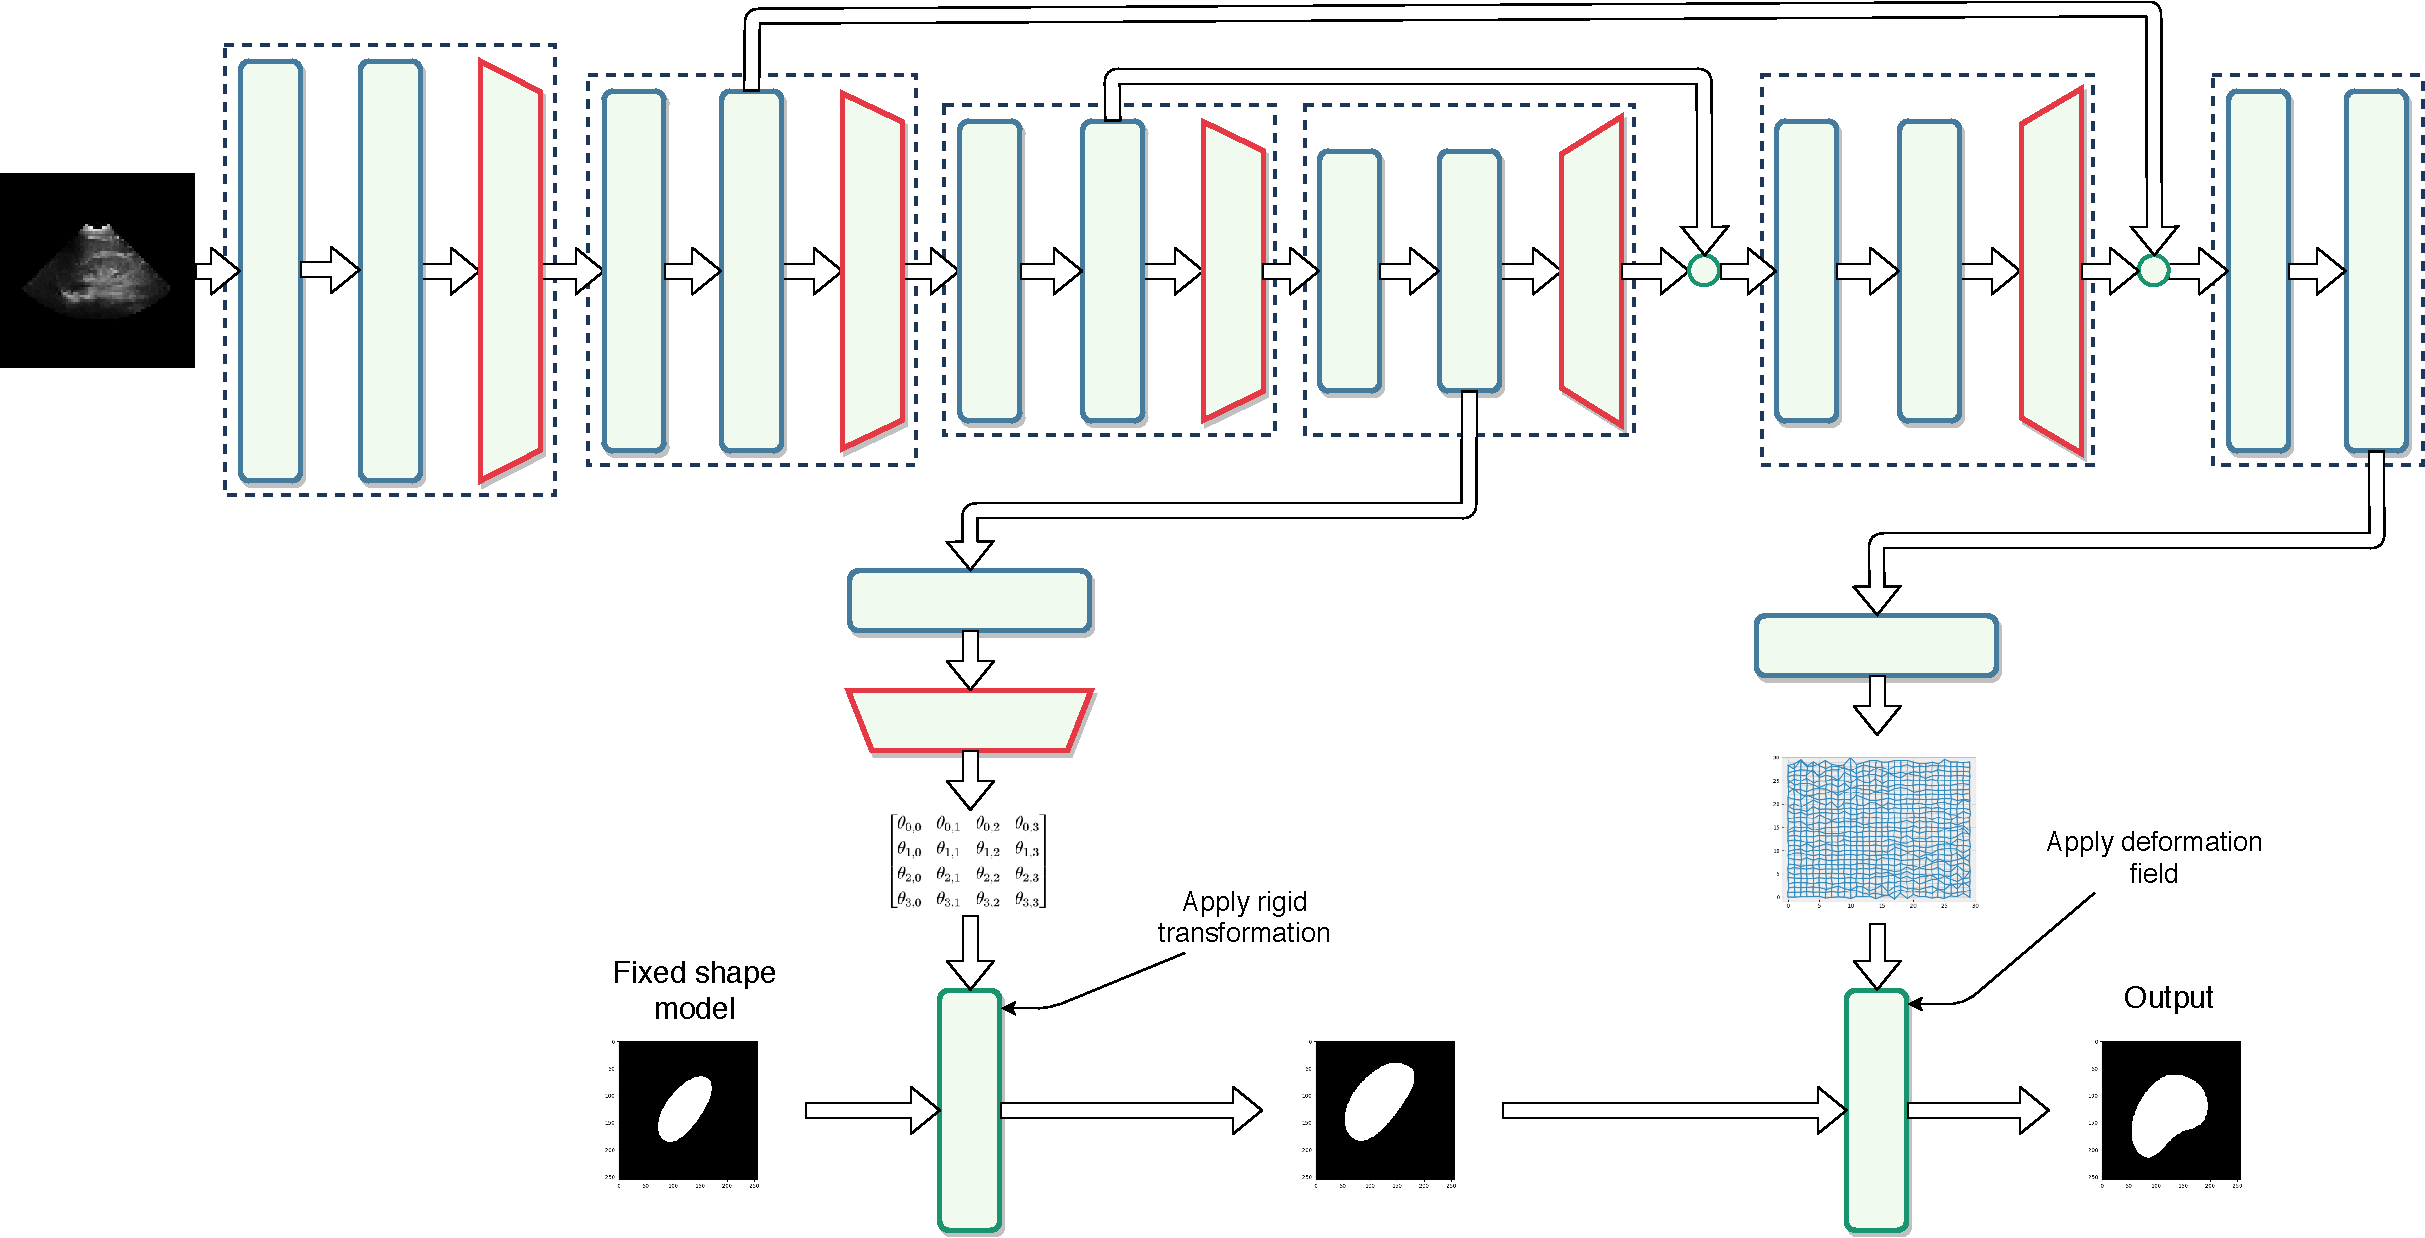
\includegraphics[width=\textwidth]{img_seg/deformation_network}
    \caption{Segmentation network that predicts a geometric transformation and a deformation field to deform a shape model.}
    \label{fig:deform_network}
\end{figure}

Figure~\ref{fig:deform_network} presents the process. The network predict a geometric transformation and a deformation field from the image, which are applied to a fixed shape model. The deformed shape model then corresponds to the correct segmentation for the image. The shape model is simply the ground truth segmentation from an image not included in the training, validation or test sets.

The next sections explains how to predict and apply the transformation and the deformation field.

\subsection{Predicting a geometric transformation}

A geometric transformation for 3D images is represented by a $4 \times 4$ matrix, meaning a total of 16 parameters that can be predicted. Directly predicting those parameters remove control on the kind of transformation that are predicted. In our case, we chose to predict instead translation, rotation and scaling parameters. 

Three parameters are predicted for the translation on each axis, giving the following translation matrix $T$:
\begin{equation*}
    T = 
    \begin{bmatrix}
        1 & 0 & 0 & t_x \\
        0 & 1 & 0 & t_y \\
        0 & 0 & 1 & t_z \\ 
        0 & 0 & 0 & 1
    \end{bmatrix}
\end{equation*}

The scaling matrix $S$ is built from three more parameters:
\begin{equation*}
    S = 
    \begin{bmatrix}
        s_x & 0 & 0 & 0 \\
        0 & s_y & 0 & 0 \\
        0 & 0 & s_z & 0 \\ 
        0 & 0 & 0 & 1
    \end{bmatrix}
\end{equation*}

Finally, we have one rotation matrix in each direction ($R_x$, $R_y$ and $R_z$) built from one parameter each:
\begin{align*}
    R_x &= 
    \begin{bmatrix}
        1 & 0 & 0 & 0 \\
        0 & \cos{r_x} & -\sin{r_x} & 0 \\
        0 & \sin{r_x} & \cos{r_x} & 0 \\ 
        0 & 0 & 0 & 1
    \end{bmatrix} \\
    R_y &= 
    \begin{bmatrix}
        \cos{r_y} & 0 & - \sin{r_y} & 0 \\
        0 & 1 & 0 & 0 \\
        \sin{r_y} & 0 & \cos{r_y} & 0 \\ 
        0 & 0 & 0 & 1
    \end{bmatrix} \\
    R_z &= 
    \begin{bmatrix}
        \cos{r_z} & -\sin{r_z} & 0 & 0 \\
        \sin{r_z} & \cos{r_z} & 0 & 0 \\
        0 & 0 & 1 & 0 \\ 
        0 & 0 & 0 & 1
    \end{bmatrix}
\end{align*}

We also need to center the image around zero before applying the rotations, which requires no parameters except knowing the center of the image:
\begin{equation*}
    C_+ = 
    \begin{bmatrix}
        1 & 0 & 0 & c_x \\
        0 & 0 & 0 & c_y \\
        0 & 0 & 0 & c_z \\ 
        0 & 0 & 0 & 1
    \end{bmatrix}
    \mkern20mu
    C_- = 
    \begin{bmatrix}
        1 & 0 & 0 & -c_x \\
        0 & 0 & 0 & -c_y \\
        0 & 0 & 0 & -c_z \\ 
        0 & 0 & 0 & 1
    \end{bmatrix}
\end{equation*}

From these matrices, the geometric transformation $G$ applied to the shape model is the following:
\begin{equation}
    G = T \cdot C_+ \cdot R_z \cdot R_y \cdot R_x \cdot S \cdot C_-
\end{equation}

The prediction of the 9 required parameters is done by a convolutional layer with 9 $1 \times 1 \times 1$ filters, followed by an average pooling layer of the size of the feature maps. 

\subsection{Predicting a deformation field}

The deformation field are predicted from a convolutional layer with 3 $3 \times 3 \times 3$ filters, one filter per dimension. Each field is then smoothed with a $3 \times 3 \times 3$ mean filter, before being resized to the shape model size with a tri-linear interpolation. This resizing step allows predicting deformation fields at a lower resolution than the shape model, saving time and parameters to learn.

% While no constraints are applied to the fields in the end, we investigated adding an $L_2$ penalty term to the deformation fields $F$ in the loss function:
% \begin{equation}
%     P = \lambda \sum_x \left( F - I \right)(x)^2
% \end{equation}

% This resulted in a drastic decrease in performance

\subsection{Distance map and loss}

- Distance map and appropriate loss

%%%%%%%%%%%%%%%%%%%%%%%%%%%%%%%%%%%%%%%%%%%%%%%%%%%%%%%%%%%%%%%%%%%%%%%%%%%%%%%%%%%%%%%%%%%%%%%
\section{Application to the segmentation of the kidney in 3D-US}

- dataset and preprocessing

TODO:
\begin{itemize}
    \item Compare global transfo alone, defo field alone, global + field
\end{itemize}


